\documentclass{article}
\usepackage[english]{babel}
\usepackage[utf8]{inputenc}
\usepackage{fancyhdr}
\usepackage{geometry}
\usepackage{enumitem}
\usepackage{amsmath}
\usepackage{graphicx}
\usepackage{tcolorbox}
\usepackage{amssymb}
\usepackage[thinc]{esdiff}
\usepackage{float}

\geometry{letterpaper, portrait, margin=1in}
\graphicspath{ {images/}  }
\pagestyle{fancy}
\fancyhf{}
\lhead{Keerthik Muruganandam}
\rhead{Hollingsworth Winter Assignment}

\begin{document}

\begin{center}
\textbf{Question 1}
\end{center}

\begin{enumerate}[label=\textbf{WS \arabic*}]

\item What is the slope of the secant line through the points $(a\text{, } f(a)) \text{ and } (a+h\text{, } f(a+h))$?

The formula for the slope of the line segment between two points $(x_1\text{, } y_1) \text{ and } (x_2, y_2)$ is
\[\frac{y_2-y_1}{x_2-x_1}\]
Thus the slope of the secant line is
\[\frac{f(a+h)-f(a)}{a+h-a}=\frac{f(a+h)-f(a)}{h}\]
That is in the form of the MVT so we know that the slope of the secant line is the derivative of some point c within $(a,a+h)$
\[f^\prime(c)=\frac{f(b)-f(a)}{b-a} \text{ in } (a\text{ , }b)\text{ and differentiable in } [a,b]\text{.}\]

\item What is the slope of the tangent line to the graph
of $f(x)$ at the point $x=\text{a}$?

 The limit definition of the derivative is
\[\lim_{h \to 0} {\frac{f(x+h)-f(x)}{h}}\]
So the slope of the tangent line to the graph of $f(x)$ at the point $x=a$ is
\[\lim_{h \to 0} {\frac{f(a+h)-f(a)}{h}}\]

\item Use a calculator to compute $\sqrt{4.1}$. How does this compare to our estimate? Was our approximation an overestimate or an underestimate?

The calculator computes $\sqrt{4.1}$ as $2.02484567313$. Compared to our estimate the real value is slightly under our estimate. The approximation was an overestimate.

\item Explain how concavity relates to the linearization of $f(x)$ being an overestimate or an underestimate.

Because $f(x)$ was concave down, the graph curves away from the tangent line in a negative fashion because the downwards concavity means that the slope of the tangent lines will be decreasing so the function flattens out in the horizontal rather than the vertical.Therefore the linear approximation will be a slight overestimate because the functions outputs increase slower than the linear function's outputs.Conversely, if a function if concave up, the outputs will increase slightly faster than the line and it will be and underestimate.
\item Use Newton's method to approximate the zero of
$f(x) = e^x - 2$ using an initial guess $x_\text{0}=1$ .

\begin{align}
x_0 &= 1 \\
x_1 &= x_0-\frac{f(x_0)}{f^\prime(x_0)}=1-\frac{\text{e}-2}{\text{e}}\approx0.735758882343 \\
x_2 &= x_1-\frac{f(x_1)}{f^\prime(x_1)}\approx0.735758882343-\frac{\text{e}^0.735758882343-2}{\text{e}^0.735758882343}\approx0.694042299919 \\
x_3 &= x_2-\frac{f(x_2)}{f^\prime(x_2)}\approx0.694042299919-\frac{\text{e}^0.694042299919-2}{\text{e}^0.694042299919}\approx0.69314758106 \\
x_4 &= x_3-\frac{f(x_3)}{f^\prime(x_2)}\approx0.69314758106-\frac{\text{e}^0.69314758106-2}{\text{e}^0.69314758106}\approx0.69314718056
\end{align}

\end{enumerate}

\newpage

\begin{center}
\textbf{Question 2}
\end{center}


The graph of the function $f(x)$ is shown below.
\begin{figure}[H]
  \centering
  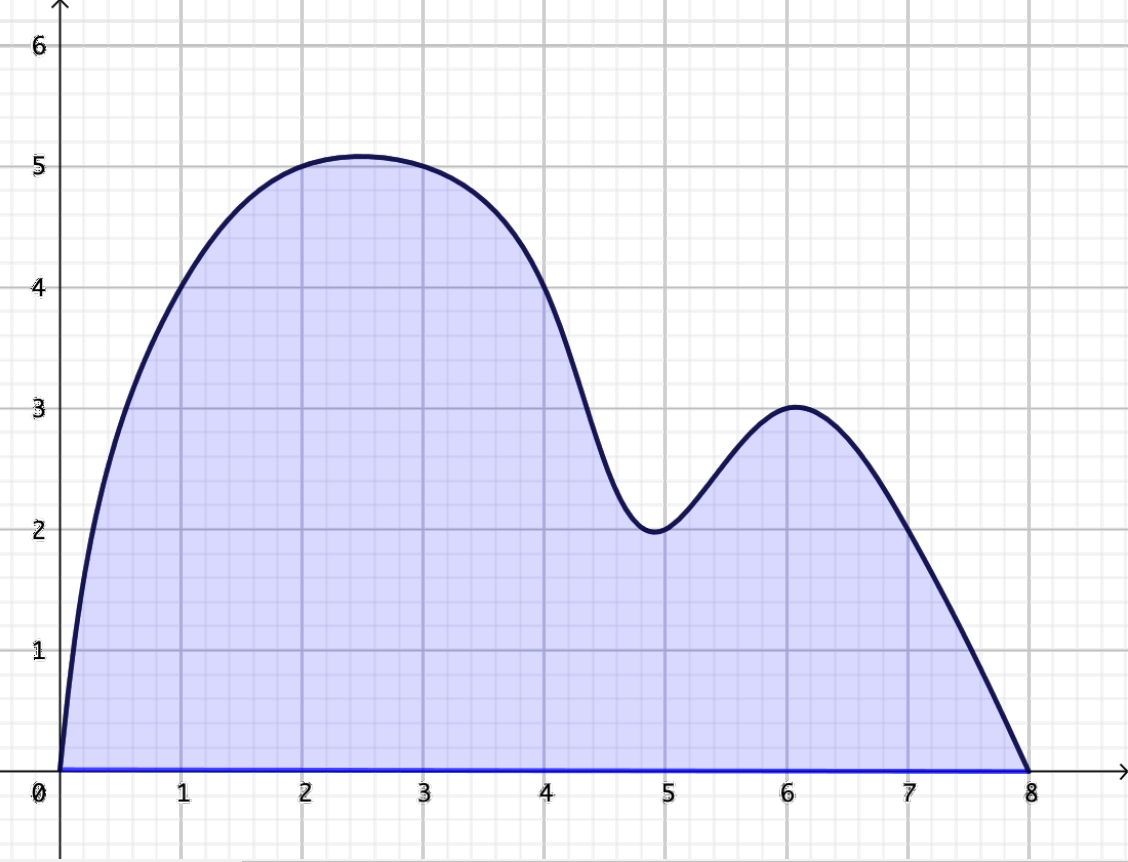
\includegraphics[width=.6\linewidth]{base}
\end{figure}
\begin{enumerate}[label=(\alph*)]
\item Estimate the area of the shaded region using 4 rectangles and right endpoints. \\
\newline
If we simulate this and sketch this out we get the figure
\begin{figure}[H]
\centering
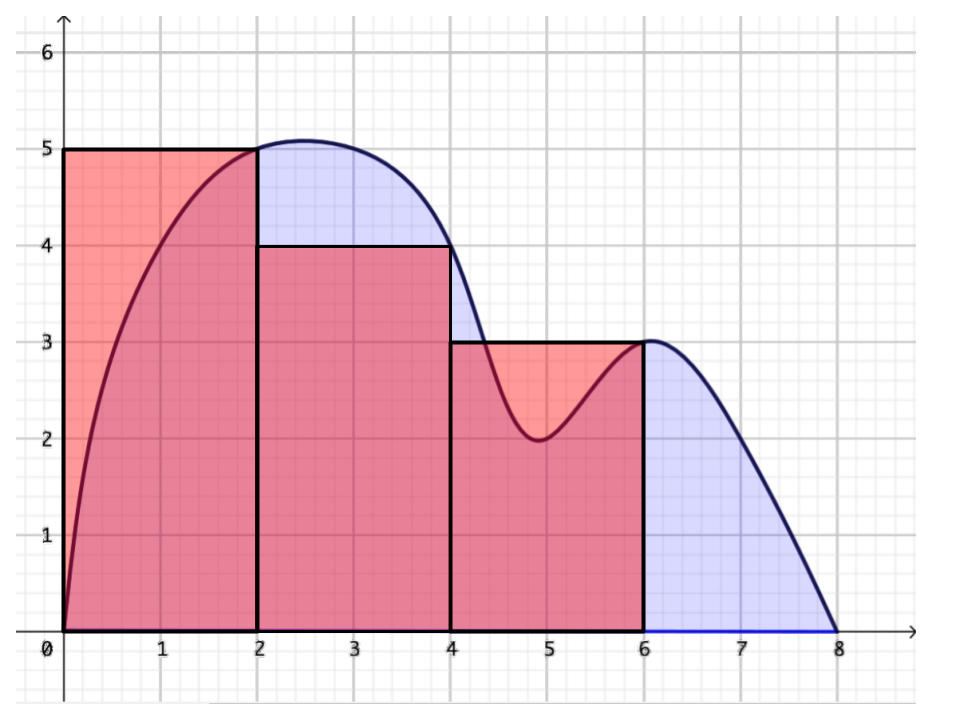
\includegraphics[width=.6\linewidth]{endpoint}
\end{figure}
We can estimate the area of the shaded squares with expression
\[2\cdot f(8)+2\cdot f(6)+ 2\cdot f(4)+ 2\cdot f(2)=\]
\[2\cdot0+2\cdot3+2\cdot 4+2\cdot 5=24\]
\newpage
\item Estimate the area of the shaded region using 8 rectangles and left endpoints. \\
\newline
If we sketch out the 8 rectangles we get the figure
\begin{figure}[H]
\centering
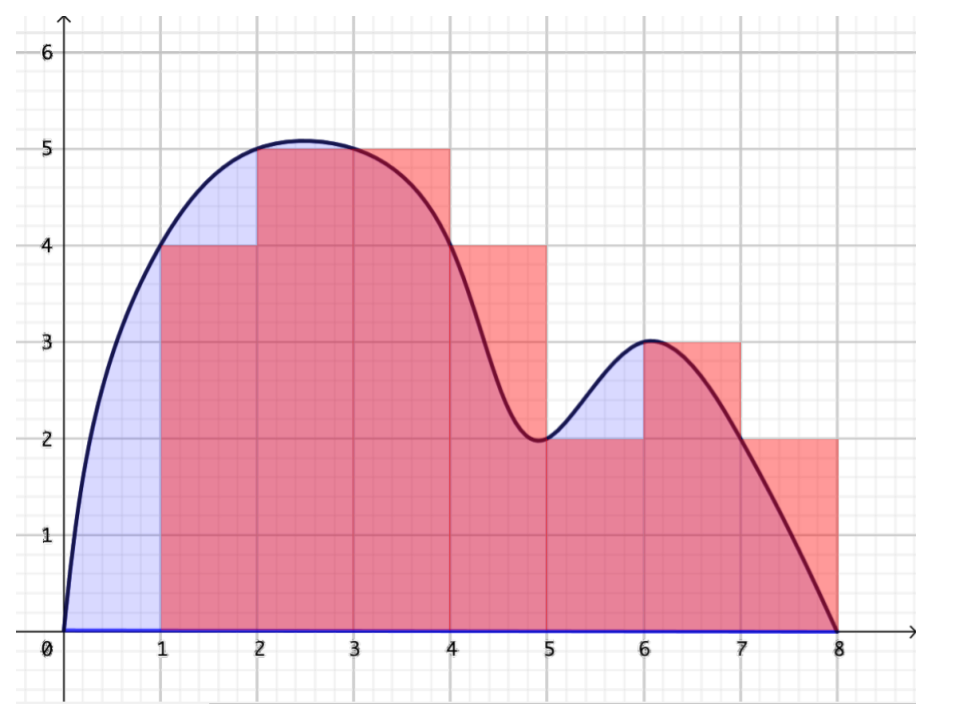
\includegraphics[width=.6\linewidth]{endnot}
\end{figure}
The estimate of the area of the shaded region is
\[4\cdot1+5\cdot1+5\cdot1+4\cdot1+2\cdot1+3\cdot1+2\cdot1= 25\]

\item Which estimate do you think is more accurate?
\par
I think that when we estimated with 8 rectangles was better because the rectangles more closely matched the shape of the figure and also because in the limit definition of the integral the limit is as $n$ approaches infinity where n is the number of rectangles in a Riemann sum of the area which means that the estimate becomes more accurate as the number of rectangles increases.Therefore the one with the more rectangles should be, theoretically, more accurate. That's why I chose the estimate using 8 rectangles as the one that was more accurate.

\newpage

\begin{center}
\textbf{Question 3} \\
Calculate the integral below using the limit definition of the definite integral.
\[\int_{-1}^4 \! (1+2x) \, \text{d}x\]
\end{center}

The limit definition of the integral is
\[\int_a^b \!f(x) \, \text{d}x = \lim_{n \to \infty} {\sum_{i=1}^{n} f(x_i)\Delta x}\]
First we need to find $\Delta x$ and $x_i$. $\Delta x$ is equal to $\dfrac{b-a}{n}$. Solving we get
\[\frac{b-a}{n}=\frac{4-(-1)}{n}=\frac{5}{n}=\Delta x\]
Next we can find the value of $x_i$ with the expression $a-i\cdot\Delta x$. Now we substitute to solve for $x_i$.
\[a-i\cdot\Delta x=-1+i(\frac{5}{n})=\frac{5}{n}i-1\]
The next step is to calculate $f(x_i)\Delta x$.
\[f(\frac{5}{n}i-1)\frac{5}{n}=(1+2(\frac{5i}{n}-1))\frac{5}{n}=(\frac{10}{n}i-1)\frac{5}{n}=\frac{50}{n^2}i-\frac{5}{n}\]
We take the sum of the expression we found above to get the summation
\begin{align*}
\sum_{i=1}^n {\left(\frac{50}{n^2}i-\frac{5}{n}\right)}&=\sum_{i=1}^n {\left(\frac{50}{n^2}i\right)}-\sum_{i=1}^n {\left(\frac{5}{n}\right)} \\
&=\frac{50}{n^2}\sum_{i=1}^n {i} - \frac{5}{n}\sum_{i=1}^{n} {1} \\
&=\frac{50}{n^2}\cdot\frac{n(n+1)}{2}-\frac{5}{n}\cdot 5 \\
&=\frac{50(n+1)}{2n}-5 \\
\end{align*}
Simplifying this, we are almost ready to complete the entire expression.
\[\frac{50n+50}{2n}-\frac{2n\cdot5}{1\cdot2n}=\frac{50n+50-10n}{2n}=\frac{40n}{2n}+\frac{50}{2n}=20+\frac{25}{n}\]
Finally we take the limit as $n$ approaches infinity of our result.
\[\lim_{n \to \infty} {20 +\frac{25}{n}}=\lim_{n \to \infty} {20} + \lim_{n \to \infty} {\frac{25}{n}}= 20 + 0=0\]
Thus, our final answer is 0.
\[\int_{-1}^4 \! (1+2x) \, \text{d}x=0\]

\newpage

\begin{center}
\textbf{Question 4} \\
Calculate the integral below using the limit definition of the definite integral.
\[\int_{0}^2 \! (x^2+5) \, \text{d}x\]
\end{center}

Once more we utilize the limit definition of a definite integral which is
\[\int_a^b \!f(x) \, \text{d}x = \lim_{n \to \infty} {\sum_{i=1}^{n} f(x_i)\Delta x}\]
Following the same pattern we need to find $\Delta x$ and $x_i$.
\[\Delta x = \frac{b-a}{n} = \frac{2-0}{n} = \frac{2}{n}\]
\[x_\text{i} = a+i\Delta x= 0+i\frac{2}{n}=\frac{2}{n}i\]
The next step is to evaluate $f(x_\text{i})\Delta x$.
\[\left({\left(\frac{2}{n}\right)}^2+5\right)\frac{2}{n}=\left(\frac{4}{n^2}i^2+5\right)\frac{2}{n}=\frac{8}{n^3}i^2+\frac{10}{n}\]
Then we take the sum of the terms after separating the terms and taking out the constants.
\begin{align*}
\sum_{i=1}^n {\left(\frac{8}{n^3}i^2+\frac{10}{n}\right)} &=\sum_{i=1}^n {\left(\frac{8}{n^3}i^2\right)}-\sum_{i=1}^n {\left(\frac{10}{n}\right)} \\
&=\frac{8}{n^3}\sum_{i=1}^n {i^2} - \frac{10}{n}\sum_{i=1}^{n} {1} \\
&=\frac{8}{n^3}\cdot\frac{n(n+1)(2n+1)}{6}-\frac{10}{n}\cdot n \\
&=\frac{4(n+1)(2n+1)}{3n^2}-10 \\
&= \frac{8n^2+12n+4}{3n^2}-10\\
&= \frac{8n^2+12n+4+30n^2}{3n^2} \\
&=\frac{38n^2+12n+4}{3n^2} \\
&=\frac{38}{3}+\frac{4}{n}+\frac{4}{3n^2}
\end{align*}
Now that we have our simplified summation we can take the limit as n approaches infinity of it.
\begin{align*}
\lim_{n\to\infty} {\left(\frac{38}{3}+\frac{4}{n}+\frac{4}{3n^2}\right)} &= \lim_{n\to\infty} \frac{38}{3} \lim_{n\to\infty} \frac{4}{n} \lim_{n\to\infty} {4}{3n^2} \\
&= \frac{38}{3}+\frac{4}{\infty}+\frac{4}{\infty} \\
&= \frac{38}{3}+0+0 \\
&=\frac{38}{3}
\end{align*}
Our answer is $\dfrac{38}{3}$.
\[\int_{0}^2 \! (x^2+5) \, \text{d}x=\frac{38}{3}\]

\end{enumerate}


\end{document}
